\chapter{Fundamentação Teórica}
\label{ch:identificador}
	\begin{resumocapitulo}
		Este capítulo aborda os fundamentos teóricos necessários para a análise do consumo de café no Brasil usando machine learning, destacando bibliotecas essenciais de Python. Pandas facilita a análise de dados com configurações personalizáveis (Voitto, 2021). Matplotlib permite a criação de gráficos e visualizações de dados através de uma interface orientada a objetos (Medium, 2020). Seaborn melhora a aparência dos gráficos, tornando-os mais polidos e intuitivos (Voooo, 2017). Essas ferramentas são cruciais para a manipulação e visualização eficaz de dados, fundamentando a aplicação de machine learning no estudo do consumo de café.
.
	\end{resumocapitulo}
	\section{Visão Geral}
		Para analisar o consumo de café no Brasil com técnicas de machine learning, é essencial utilizar ferramentas robustas para manipulação e visualização de dados. Três bibliotecas de Python destacam-se nesse contexto: Pandas, Matplotlib e Seaborn.

	\section{Funções utilizadas}
	\label{sec:identificao}
      
		% Lista numerada
		\begin{enumerate}
			\item CONFIGURANDO A TABELA QUE SERÁ UTILIZADA
			\item Cerregando a biblioteca pandas e atribui um alias chamado "pd"
                \item Realizando a conexão com o google Drive
                \item Realizando a leitura do arquivo csv
                \item Criando tabela de colunas
                \item Criando o gráfico de colunas
                \item Adicionando título e rótulos aos eixos
                \item Mostrando o gráfico
                \item Supondo que "df menor" seja o seu DataFrame com as colunas especificadas
                \item Tavez precise ajustar o nome das colunas de acordo com o seu DataFrame
                \item Agrupando por região e produto e somando as vendas
                \item Encontrando o produto mais vendido em cada região
                \item Adicionando título e rótulos aos eixos
                \item Rotaciona os rótulos do eixo x para melhor visualização
                \item Exibindo o produto mais vendido em cada região
                \item Filtrando os dados apenas para a região de Vila Prudente
                \item Agrupando por tipo de café e somando as vendas
                \item Ordenando os dados pelo total de vendas (do maior para o menor)
                \item Filtrando os dados apenas para a região de Santo André
                \item Filtrando os dados apenas para a região de Osasco
                \item Filtrando os dados apenas para a região do Brás
                \item Define o tipo de café
                \item Filtra os dados para o tipo de café específico
                \item grupando por tipo de café e somando os valores das vendas
                \item Agrupando por região e tipo de café e somando os valores das vendas
                
		\end{enumerate}

 
% % %         \section{Cafés mais vendidos por valor em cada região.}
% % % \label{sec:figura}
% % A Figura~\ref{figuras/configuraçao-introduçao.png} Ao investigarmos os cafés mais populares em cada região, mergulhamos no mundo dos gostos e preferências dos consumidores. Observamos não apenas números, mas também as histórias por trás de cada xícara.
% % \begin{figure}[!ht]
% % 	{\centering
% % 		\caption{Descrição da figura.}
% % 		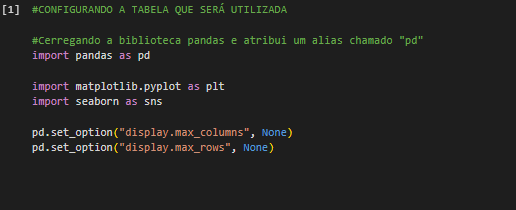
\includegraphics[width=1.0\textwidth]{figuras/configuraçao-introduçao.png}
% % 		\label{figuras/configuraçao-introduçao.png
% % 		\fonte{Google Colab}
% % 	}
% % \end{figure} \\ \\ \\ \\ \\ \\ \\ 
% }

% 		% % Lista numerada
% 		% \begin{enumerate}
% 		% 	\item Bla
% 		% 	\item Bla
% 		% \end{enumerate}
% \




		% % Lacuna de pesquisa - um bloco para cada lacuna
		% \begin{lacuna}
		% \label{lacuna:lacuna1}
		% 	Descrever aqui a lacuna de pesquisa. Se tiver mais que uma, criar outro bloco.
		% \end{lacuna}
	
		% % Pergunta de pesquisa - um bloco para cada pergunta
		% \begin{pergunta}
		% \label{pergunta:pergunta_1}
		% 	Aqui vai a pergunta de pesquisa 1.
		% \end{pergunta}

		% \begin{pergunta}
		% \label{pergunta:pergunta_2}
		% 	Aqui vai a pergunta de pesquisa 2.
		% \end{pergunta}	